%\documentclass{article}
%\usepackage{amsfonts,amssymb,graphics,amsmath,amsthm,comment}
%\usepackage[mathscr]{euscript}
%\usepackage{tikz}
%
%\begin{document}
%
%\begin{figure}[h]
%\begin{center}





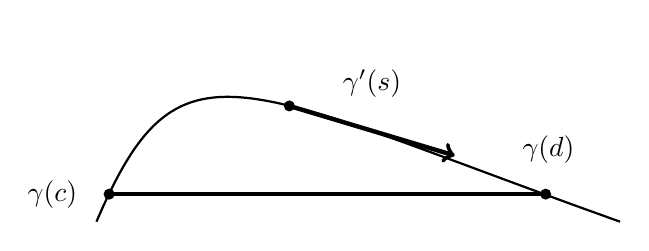
\begin{tikzpicture}[inner sep=0pt,thick,
        dot/.style={fill=black,circle,minimum size=4pt}, scale=0.7]

\draw[ultra thick, -] (-4.27,0) -- (3.65,0);
\draw[-] (-4.5,-0.5) .. controls (-3,3) and (-2,2) .. (5,-0.5);
\draw[ultra thick, ->] (-1,1.6) -- (2,0.7);
%\draw[ultra thick, ->] (-1,-3) -- (2,-1.7);


\node[dot] at (-4.27,0) {};
\node[dot] at (3.65,0) {};
\node[dot] at (-1,1.6) {};

\node at (-5.3, 0) {$\gamma(c)$};
\node at (3.7, 0.8) {$\gamma(d)$};
%\node at (0.8, -3) {$\mathbf{u}_0$};
\node at (0.5, 2) {$\gamma'(s)$};

\end{tikzpicture}





%\end{center}
%\caption{Illustration of Sublemma}
%\end{figure}
%
%\end{document}